\documentclass[11pt,a4paper]{article}

% ==============================================================================
% PAQUETES BASE (100% compatible con Overleaf / pdfLaTeX)
% ==============================================================================
\usepackage[utf8]{inputenc}
\usepackage[T1]{fontenc}
\usepackage[spanish,es-tabla]{babel}
\usepackage{lmodern}
\usepackage[margin=2.5cm, headheight=15pt]{geometry}
\usepackage{graphicx}
\usepackage{float}
\usepackage{booktabs}
\usepackage{tabularx}
\usepackage{longtable}
\usepackage{array}
\usepackage[table]{xcolor}
\usepackage{titlesec}
\usepackage{fancyhdr}
\usepackage{enumitem}
\usepackage{caption}
\usepackage{hyperref}

% ==============================================================================
% ESTILOS, COLORES Y ENCABEZADOS
% ==============================================================================
\definecolor{PrimaryNavy}{HTML}{1B365D}
\definecolor{AccentBlue}{HTML}{2C5AA0}
\definecolor{LightTint}{HTML}{F2F5F9}
\definecolor{BorderGray}{HTML}{D0D7DE}

\hypersetup{
    colorlinks=true,
    linkcolor=PrimaryNavy,
    urlcolor=AccentBlue,
    pdftitle={Entrega Nro. 1 - Sistema Web y Movil SST Municipalidad Distrital de Wanchaq},
    pdfauthor={Cesar Andersson Saire Hancco, Andy Yoseph Quispe Huanca, Abelardo Ttito Quispe, Jean Marco Pacha Quispe}
}

\graphicspath{{imagenes/}}

\pagestyle{fancy}
\fancyhf{}
\fancyhead[L]{\small\color{gray} Ingeniería de Software I --- Proyecto SST Wanchaq}
\fancyhead[R]{\small\color{gray} Entrega N.\textsuperscript{o} 1}
\fancyfoot[C]{\small\thepage}
\renewcommand{\headrulewidth}{0.4pt}

\titleformat{\section}
  {\Large\bfseries\color{PrimaryNavy}}
  {}
  {0em}
  {}[\vspace{-0.4em}\color{PrimaryNavy}\titlerule]

\titleformat{\subsection}
  {\large\bfseries\color{AccentBlue}}
  {}
  {0em}
  {}

\titleformat{\subsubsection}
  {\normalsize\bfseries\color{PrimaryNavy}}
  {}
  {0em}
  {}

\captionsetup{
    font=small,
    labelfont={bf,color=PrimaryNavy},
    justification=centering
}

\setlength{\parskip}{0.5em}
\setlength{\parindent}{0pt}

\newcolumntype{L}[1]{>{\raggedright\arraybackslash}p{#1}}
\newcolumntype{C}[1]{>{\centering\arraybackslash}p{#1}}
\newcolumntype{Y}{>{\raggedright\arraybackslash}X}

% ==============================================================================
% INICIO DEL DOCUMENTO (SIN CARÁTULA)
% ==============================================================================
\begin{document}

% Nota: Si deseas incluir un índice automático antes del Capítulo I, descomenta las siguientes líneas:
% \tableofcontents
% \newpage

% ==============================================================================
% CAPÍTULO I: DATOS GENERALES DEL PROYECTO
% ==============================================================================
\section*{I. DATOS GENERALES DEL PROYECTO}
\addcontentsline{toc}{section}{I. Datos Generales del Proyecto}

\subsection*{1.1. Título del Proyecto}
\addcontentsline{toc}{subsection}{1.1. Título del Proyecto}

\textbf{Diseño e Implementación de un Sistema Web y Móvil para la Gestión, Acreditación Geolocalizada e Impacto Sostenible de Capacitaciones en Seguridad y Salud en el Trabajo (Ley N.\textsuperscript{o} 29783) en el Personal Operativo de la Municipalidad Distrital de Wanchaq.}

\subsection*{1.2. Objetivos del Proyecto}
\addcontentsline{toc}{subsection}{1.2. Objetivos del Proyecto}

\subsubsection*{Objetivo General}
Diseñar e implementar una plataforma web y móvil integral para la gestión, seguimiento en campo, certificación digital y evaluación del impacto sostenible de los programas obligatorios de capacitación en Seguridad y Salud en el Trabajo (SST) dirigidos al personal operativo de la Municipalidad Distrital de Wanchaq (Cusco), optimizando la asignación de instructores, el control de asistencia geolocalizada, la emisión automatizada de certificados verificables con código QR y el cumplimiento normativo mediante la metodología ágil SCRUM.

\subsubsection*{Objetivos Específicos}
\begin{enumerate}[leftmargin=1.5em, itemsep=0.3em]
    \item \textbf{Gestionar eficientemente el padrón de capacitandos, instructores, cursos SST y sedes operativas} del distrito de Wanchaq (Palacio Municipal, Planta de Maestranza, Vivero Municipal y frentes de obra pública), categorizando al personal por área operativa y garantizando el cumplimiento de la Ley de Protección de Datos Personales (Ley N.\textsuperscript{o} 29733).
    \item \textbf{Implementar un módulo móvil en Flutter para el control de asistencia en campo y seguimiento en tiempo real}, integrando códigos QR dinámicos temporales y validación de geolocalización por geocerca GPS con soporte \textit{offline-first} para cuadrillas con conectividad intermitente.
    \item \textbf{Automatizar la evaluación de aprendizaje y la generación de certificados y carnets digitales verificables} en formato PDF con código QR único, asegurando la autenticidad ante inspecciones internas o auditorías externas sin riesgo de falsificación.
    \item \textbf{Proveer un dashboard analítico de cumplimiento normativo e impacto sostenible}, permitiendo monitorear la meta legal de cuatro (4) capacitaciones anuales por trabajador (Ley N.\textsuperscript{o} 29783), exportar el registro oficial en formato R.M. N.\textsuperscript{o} 050-2013-TR (auditable ante SUNAFIL/SERVIR) y cuantificar el impacto social, económico y ambiental.
\end{enumerate}

\subsection*{1.3. Alcance del Sistema}
\addcontentsline{toc}{subsection}{1.3. Alcance del Sistema}

El sistema abarca la gestión del ciclo de vida completo de las capacitaciones de Seguridad y Salud en el Trabajo (SST) dentro del caso de estudio de la \textbf{Municipalidad Distrital de Wanchaq}, desde la planificación del Plan Anual de SST hasta la emisión de certificados verificables y la generación de reportes gerenciales e indicadores de sostenibilidad. Aunque la validación corresponde a la Municipalidad Distrital de Wanchaq, la arquitectura se diseña de manera modular y parametrizable (Sedes, Áreas Operativas y Cuadrillas), permitiendo su escalabilidad hacia cualquier gobierno local o entidad pública de la región Cusco.

\subsubsection*{Módulos Incluidos en el Alcance}
\begin{itemize}[leftmargin=1.5em, itemsep=0.25em]
    \item \textbf{Módulo 1 --- Gestión de Usuarios, Roles y Zonas/Sedes Operativas:} Autenticación JWT, control de acceso basado en roles (Administrador SST, Instructor/Capataz, Personal Operativo), padrón de trabajadores por gerencia/área (Limpieza Pública, Parques y Jardines, Obras Públicas, Serenazgo), georreferenciación de sedes con geocercas GPS y gestión del consentimiento informado LPDP.
    \item \textbf{Módulo 2 --- Gestión del Catálogo de Capacitaciones SST y Materiales:} Administración de cursos obligatorios (IPERC, Uso de EPPs, Primeros Auxilios, Ergonomía, Manejo Defensivo, Simulacros), carga de temarios y guías descargables en PDF, asignación de instructores y programación de sesiones por cuadrillas sin cruce de horarios.
    \item \textbf{Módulo 3 --- Monitoreo, Control de Asistencia y Geolocalización Móvil:} Generación de códigos QR dinámicos con expiración corta por sesión, marcado de asistencia desde la aplicación móvil Flutter validando la ubicación GPS puntual dentro de la geocerca autorizada, monitoreo en tiempo real y sincronización \textit{offline-first}.
    \item \textbf{Módulo 4 --- Aplicación Móvil para Capacitandos (Personal Operativo):} Consulta de sesiones programadas, barra de progreso respecto a la cuota legal anual (4 capacitaciones/año), notificaciones push de recordatorio, acceso a material de estudio y descarga de carnets/certificados digitales.
    \item \textbf{Módulo 5 --- Sistema de Evaluaciones, Certificación Digital y Alertas:} Cuestionarios automatizados (pre-test y post-test) con calificación inmediata, alertas de inasistencia o incumplimiento próximo de la cuota anual, y generación automatizada de certificados/carnets PDF firmados institucionalmente con código QR de verificación pública.
    \item \textbf{Módulo 6 --- Analítica, Cumplimiento Normativo e Impacto Sostenible (Dashboard):} Panel interactivo de cobertura SST por área municipal, tasa de aprobación, exportación del Registro Oficial en formato \textbf{R.M. N.\textsuperscript{o} 050-2013-TR}, y cálculo de métricas sostenibles (ahorro de papel, huella de carbono evitada, horas-hombre capacitadas e inclusión laboral).
\end{itemize}

\subsubsection*{Exclusiones y Limitaciones del Alcance}
\begin{itemize}[leftmargin=1.5em, itemsep=0.2em]
    \item No incluye la integración directa con sistemas legados internos de planillas estatales (SIAF/SIGA); la carga de personal se realiza mediante los formularios del sistema o importación controlada.
    \item No contempla rastreo GPS continuo en segundo plano de los trabajadores; la geolocalización se captura exclusivamente en el instante puntual de validación de asistencia, en estricto respeto de la privacidad y la Ley N.\textsuperscript{o} 29733.
\end{itemize}

\subsection*{1.4. Justificación del Proyecto}
\addcontentsline{toc}{subsection}{1.4. Justificación del Proyecto}

El distrito de Wanchaq constituye uno de los polos urbanos más dinámicos y densos de la provincia del Cusco, demandando la operación continua de cuadrillas municipales de Limpieza Pública, Mantenimiento de Parques y Jardines, Serenazgo e Infraestructura/Obras Públicas en distintos frentes de trabajo (Av. de la Cultura, Marcavalle, Magisterio, Progreso, Planta de Maestranza, Vivero Municipal, entre otros).

Actualmente, el registro de capacitaciones y charlas de seguridad en entornos municipales suele ejecutarse mediante \textbf{planillas físicas en papel y hojas de cálculo aisladas}, generando las siguientes problemáticas críticas:
\begin{enumerate}[leftmargin=1.5em, itemsep=0.25em]
    \item \textbf{Riesgo de sanciones legales:} La \textbf{Ley N.\textsuperscript{o} 29783} y su Reglamento (\textbf{D.S. N.\textsuperscript{o} 005-2012-TR}) obligan al empleador a impartir al menos \textbf{cuatro (4) capacitaciones anuales} por trabajador y conservar registros auditables durante 5 años según los formatos referenciales de la \textbf{R.M. N.\textsuperscript{o} 050-2013-TR}. El extravío de hojas de asistencia expone a la entidad a observaciones de \textbf{SERVIR} y multas de \textbf{SUNAFIL}.
    \item \textbf{Falta de trazabilidad y suplantación en campo:} Al ejecutarse charlas de inducción en zonas abiertas y frentes de obra dispersos, resulta difícil verificar fehacientemente la presencia física del trabajador en el horario y lugar programado.
    \item \textbf{Retraso y vulnerabilidad documental:} La emisión manual de constancias demora semanas y carece de mecanismos de verificación instantánea ante supervisores de obra, facilitando la falsificación de certificados.
    \item \textbf{Invisibilidad del impacto y alto consumo de papel:} No se cuenta con indicadores consolidados en tiempo real sobre tasas de aprendizaje, brechas por gerencia ni sobre el impacto ambiental derivado del uso intensivo de papelería.
\end{enumerate}

La implementación de la plataforma propuesta digitaliza el formato R.M. N.\textsuperscript{o} 050-2013-TR con evidencia verificable (QR dinámico + geocerca GPS), fortalece la cultura preventiva del personal operativo de campo, elimina el consumo masivo de papel y provee indicadores transparentes de sostenibilidad institucional.

\subsection*{1.5. Tecnologías Utilizadas}
\addcontentsline{toc}{subsection}{1.5. Tecnologías Utilizadas}

El stack tecnológico seleccionado por el equipo se detalla en la Tabla~\ref{tab:stack}.

\begin{table}[H]
\centering
\caption{Stack tecnológico y herramientas seleccionadas para el proyecto}
\label{tab:stack}
\renewcommand{\arraystretch}{1.25}
\small
\begin{tabularx}{\textwidth}{L{3.4cm} L{4.0cm} Y}
\toprule
\rowcolor{PrimaryNavy}
\textcolor{white}{\textbf{Categoría}} & \textcolor{white}{\textbf{Tecnología}} & \textcolor{white}{\textbf{Justificación Técnica}} \\
\midrule
Backend (API REST) & Node.js + NestJS (TypeScript) & Arquitectura modular por capas e inyección de dependencias; tipado estricto y manejo ágil de JWT, PDF y QR. \\
\rowcolor{LightTint}
Frontend Web & React + TypeScript + Tailwind CSS & Componentes reutilizables ideales para dashboards interactivos con diseño responsivo rápido y consistente. \\
Aplicación Móvil & Dart + Flutter & Desarrollo multiplataforma (Android/iOS) con acceso nativo a cámara (escáner QR), sensor GPS y persistencia \textit{offline-first}. \\
\rowcolor{LightTint}
BD Relacional & PostgreSQL & Motor compatible con ACID para modelar usuarios, roles, sedes, catálogo SST, sesiones, asistencias y certificados. \\
BD NoSQL & MongoDB & Almacenamiento flexible para logs inmutables de auditoría LPDP, intentos GPS y analítica de evaluaciones. \\
\rowcolor{LightTint}
Gestión Scrum & Jira Software Cloud & Gestión del Product Backlog, Épicas, Historias de Usuario, Story Points, Sprints e integración nativa con GitHub. \\
Control de Versiones & Git + GitHub & Repositorio centralizado (\url{https://github.com/141158/sst-wanchaq-platform}) conectado a Jira. \\
\rowcolor{LightTint}
Diseño y Comunicación & Figma, Discord / WhatsApp & Prototipado colaborativo de interfaces UI/UX y coordinación de ceremonias Scrum diarias. \\
Despliegue Cloud & Vercel / Render / Railway & Despliegue continuo en la nube para el entregable final del sistema al 100\%. \\
\bottomrule
\end{tabularx}
\end{table}

\subsection*{1.6. Roles del Equipo Scrum}
\addcontentsline{toc}{subsection}{1.6. Roles del Equipo Scrum}

El equipo está conformado por cuatro (4) integrantes distribuidos según los roles del marco de trabajo Scrum (Tabla~\ref{tab:roles}).

\begin{table}[H]
\centering
\caption{Integrantes y asignación de roles del equipo Scrum}
\label{tab:roles}
\renewcommand{\arraystretch}{1.25}
\small
\begin{tabularx}{\textwidth}{L{3.8cm} C{1.6cm} L{3.1cm} Y}
\toprule
\rowcolor{PrimaryNavy}
\textcolor{white}{\textbf{Integrante}} & \textcolor{white}{\textbf{Código}} & \textcolor{white}{\textbf{Rol Scrum}} & \textcolor{white}{\textbf{Funciones Principales}} \\
\midrule
Cesar Andersson Saire Hancco & 141158 & Scrum Master & Facilita ceremonias Scrum (Planning, Dailies, Review, Retrospective), elimina bloqueos, gestiona Jira y asegura el cumplimiento de la DoD y la LPDP. \\
\rowcolor{LightTint}
Andy Yoseph Quispe Huanca & 221949 & Product Owner & Representa al Comité de SST de Wanchaq, prioriza el Product Backlog, define criterios de aceptación y valida los incrementos en cada Sprint Review. \\
Abelardo Ttito Quispe & 192430 & Developer 1 (Fullstack / Lead Backend) & Diseña e implementa la API REST en Node.js (NestJS), bases de datos PostgreSQL/MongoDB, seguridad JWT/RBAC, certificados PDF/QR y exportación R.M. 050-2013-TR. \\
\rowcolor{LightTint}
Jean Marco Pacha Quispe & 164246 & Developer 2 (Mobile / Frontend) & Desarrolla la aplicación móvil en Flutter (escaneo QR, geolocalización GPS, modo offline) y el panel web/dashboard en React + TypeScript + Tailwind CSS. \\
\bottomrule
\end{tabularx}
\end{table}

\subsection*{1.7. Público Objetivo del Sistema}
\addcontentsline{toc}{subsection}{1.7. Público Objetivo del Sistema}

\begin{itemize}[leftmargin=1.5em, itemsep=0.25em]
    \item \textbf{Administradores / Coordinadores de SST (Oficina de RRHH y Comité de SST de Wanchaq):} Planifican el calendario anual de capacitaciones, gestionan el padrón operativo, parametrizan sedes georreferenciadas y exportan reportes de auditoría.
    \item \textbf{Instructores / Ponentes / Capataces de SST:} Imparten talleres y charlas de seguridad en campo, cargan materiales de estudio, generan códigos QR dinámicos de asistencia y evalúan el aprendizaje.
    \item \textbf{Personal Operativo / Capacitandos (Limpieza Pública, Parques y Jardines, Obras Públicas y Serenazgo):} Registran su asistencia desde el dispositivo móvil, consultan su progreso legal anual, rinden evaluaciones y descargan sus certificados digitales.
    \item \textbf{Actores Externos de Verificación (Supervisores de Obra, SUNAFIL y SERVIR):} Verifican de manera pública e instantánea la validez de los certificados SST escaneando el código QR institucional.
\end{itemize}

\newpage

% ==============================================================================
% CAPÍTULO II: MÉTODO SCRUM APLICADO (BOSQUEJO - ENTREGA NRO. 1)
% ==============================================================================
\section*{II. MÉTODO SCRUM APLICADO (BOSQUEJO --- ENTREGA N.\textsuperscript{o} 1)}
\addcontentsline{toc}{section}{II. Método Scrum Aplicado}

\subsection*{2.1. Product Backlog Inicial Priorizado}
\addcontentsline{toc}{subsection}{2.1. Product Backlog Inicial Priorizado}

El Product Backlog inicial fue estructurado y priorizado directamente en \textbf{Jira Software} (Proyecto \texttt{SST-Wanchaq}, clave \texttt{SCRUM}), agrupando los \textbf{Requisitos Funcionales (RF)} en \textbf{6 Épicas} correspondientes a los módulos del sistema y \textbf{18 Historias de Usuario (HU)} estimadas con la escala de Fibonacci (\textbf{92 Story Points} totales).

\subsubsection*{A. Resumen de Épicas en Jira}

\begin{table}[H]
\centering
\caption{Épicas definidas en Jira Software mapeadas a los 6 módulos del sistema}
\label{tab:epicas}
\renewcommand{\arraystretch}{1.22}
\small
\begin{tabularx}{\textwidth}{C{1.9cm} C{1.2cm} Y C{1.8cm} L{2.8cm}}
\toprule
\rowcolor{PrimaryNavy}
\textcolor{white}{\textbf{Clave Jira}} & \textcolor{white}{\textbf{Cód.}} & \textcolor{white}{\textbf{Épica / Módulo Funcional}} & \textcolor{white}{\textbf{Prioridad}} & \textcolor{white}{\textbf{Responsable}} \\
\midrule
\texttt{SCRUM-5} & EP-1 & Módulo 1: Gestión de Usuarios, Roles y Zonas Operativas (Wanchaq) & Highest & Abelardo Ttito \\
\rowcolor{LightTint}
\texttt{SCRUM-6} & EP-2 & Módulo 2: Catálogo de Capacitaciones SST (Ley 29783) y Materiales & Highest & Andy Quispe \\
\texttt{SCRUM-7} & EP-3 & Módulo 3: Control de Asistencia Móvil, QR Dinámico y Geolocalización & Highest & Jean Marco Pacha \\
\rowcolor{LightTint}
\texttt{SCRUM-8} & EP-4 & Módulo 4: Aplicación Móvil para Personal Operativo (Capacitandos) & High & Jean Marco Pacha \\
\texttt{SCRUM-9} & EP-5 & Módulo 5: Evaluaciones Automatizadas, Alertas y Certificación QR & High & Abelardo Ttito \\
\rowcolor{LightTint}
\texttt{SCRUM-10} & EP-6 & Módulo 6: Analítica, Cumplimiento SUNAFIL e Impacto Sostenible & Medium & Cesar Saire \\
\bottomrule
\end{tabularx}
\end{table}

\subsubsection*{B. Listado Priorizado de Historias de Usuario (Requisitos Funcionales)}

{\setlength{\tabcolsep}{3.5pt}
\renewcommand{\arraystretch}{1.2}
\footnotesize
\begin{longtable}{C{1.5cm} C{0.95cm} C{0.85cm} L{5.4cm} C{1.2cm} C{0.6cm} C{1.75cm} L{1.75cm}}
\caption{Product Backlog inicial priorizado registrado en Jira Software} \label{tab:backlog} \\
\toprule
\rowcolor{PrimaryNavy}
\textcolor{white}{\textbf{Jira}} & \textcolor{white}{\textbf{ID}} & \textcolor{white}{\textbf{Épica}} & \textcolor{white}{\textbf{Historia de Usuario (Resumen)}} & \textcolor{white}{\textbf{Prioridad}} & \textcolor{white}{\textbf{SP}} & \textcolor{white}{\textbf{Sprint}} & \textcolor{white}{\textbf{Responsable}} \\
\midrule
\endfirsthead
\multicolumn{8}{c}{\tablename\ \thetable{} --- \textit{Continuación de la página anterior}} \\
\toprule
\rowcolor{PrimaryNavy}
\textcolor{white}{\textbf{Jira}} & \textcolor{white}{\textbf{ID}} & \textcolor{white}{\textbf{Épica}} & \textcolor{white}{\textbf{Historia de Usuario (Resumen)}} & \textcolor{white}{\textbf{Prioridad}} & \textcolor{white}{\textbf{SP}} & \textcolor{white}{\textbf{Sprint}} & \textcolor{white}{\textbf{Responsable}} \\
\midrule
\endhead
\bottomrule
\endfoot

\texttt{SCRUM-11} & HU-01 & EP-1 & Autenticación segura (JWT) y control de acceso por roles (RBAC) & Highest & 5 & Sprint 1 & A. Ttito \\
\rowcolor{LightTint}
\texttt{SCRUM-12} & HU-02 & EP-1 & Gestión CRUD de personal operativo de la Municipalidad de Wanchaq & Highest & 5 & Sprint 1 & A. Ttito \\
\texttt{SCRUM-13} & HU-03 & EP-1 & Configuración de sedes y zonas operativas georreferenciadas de Wanchaq & High & 3 & Sprint 1 & J. Pacha \\
\rowcolor{LightTint}
\texttt{SCRUM-14} & HU-04 & EP-1 & Consentimiento informado digital y logs de auditoría (Ley N.\textsuperscript{o} 29733 - LPDP) & High & 3 & Sprint 1 & C. Saire \\
\texttt{SCRUM-15} & HU-05 & EP-2 & Gestión del catálogo de capacitaciones SST (Ley 29783) y asignación de instructores & Highest & 5 & Sprint 2 & A. Ttito \\
\rowcolor{LightTint}
\texttt{SCRUM-16} & HU-06 & EP-2 & Gestión de temarios y materiales descargables de capacitación & High & 3 & Sprint 2 & J. Pacha \\
\texttt{SCRUM-17} & HU-07 & EP-2 & Programación de sesiones y asignación de cuadrillas de Wanchaq & High & 5 & Sprint 2 & A. Quispe \\
\rowcolor{LightTint}
\texttt{SCRUM-18} & HU-08 & EP-3 & Generación de código QR dinámico temporal por sesión de capacitación & Highest & 8 & Sprint 2 & J. Pacha \\
\texttt{SCRUM-19} & HU-09 & EP-3 & Registro de asistencia presencial vía QR y validación GPS (Geocerca) en App Flutter & Highest & 8 & Sprint 2 & J. Pacha \\
\rowcolor{LightTint}
\texttt{SCRUM-20} & HU-10 & EP-3 & Monitoreo de asistencia en tiempo real y sincronización \textit{offline-first} & High & 5 & Sprint 2 & A. Ttito \\
\texttt{SCRUM-21} & HU-11 & EP-4 & Consulta móvil de inscripciones, historial SST y calendario del trabajador & High & 5 & Sprint 3 (Backlog) & J. Pacha \\
\rowcolor{LightTint}
\texttt{SCRUM-22} & HU-12 & EP-4 & Notificaciones push de inicio de clases y acceso móvil a material interactivo & Medium & 3 & Sprint 3 (Backlog) & J. Pacha \\
\texttt{SCRUM-23} & HU-13 & EP-5 & Sistema de evaluaciones automatizadas (Pre-test y Post-test SST) & High & 5 & Sprint 3 (Backlog) & A. Ttito \\
\rowcolor{LightTint}
\texttt{SCRUM-24} & HU-14 & EP-5 & Generación automatizada de certificados y carnets PDF con verificación QR & Highest & 8 & Sprint 3 (Backlog) & A. Ttito \\
\texttt{SCRUM-25} & HU-15 & EP-5 & Alertas automatizadas de inasistencia y riesgo de incumplimiento Ley 29783 & Medium & 3 & Sprint 4 (Backlog) & A. Ttito \\
\rowcolor{LightTint}
\texttt{SCRUM-26} & HU-16 & EP-6 & Dashboard analítico de cumplimiento SST por gerencia y tasa de aprobación & High & 8 & Sprint 4 (Backlog) & J. Pacha \\
\texttt{SCRUM-27} & HU-17 & EP-6 & Exportación del Registro Oficial de Capacitación (Formato R.M. 050-2013-TR) & High & 5 & Sprint 4 (Backlog) & A. Ttito \\
\rowcolor{LightTint}
\texttt{SCRUM-28} & HU-18 & EP-6 & Panel de métricas de impacto sostenible (Ambiental, Social y Económico) & Medium & 5 & Sprint 4 (Backlog) & C. Saire \\
\end{longtable}}
\normalsize

\begin{figure}[H]
    \centering
    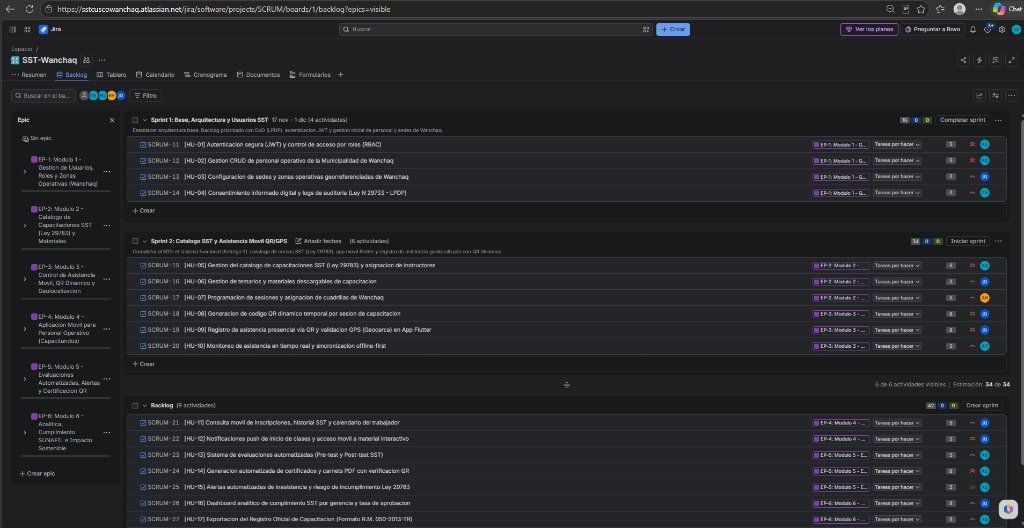
\includegraphics[width=\textwidth]{captura1_jira_backlog.jpg}
    \caption{Vista del Product Backlog inicial priorizado en Jira Software (\texttt{sstcuscowanchaq.atlassian.net}), mostrando el panel de 6 Épicas, Sprint 1 (16 SP), Sprint 2 (34 SP) y Backlog priorizado (42 SP).}
    \label{fig:jira_backlog}
\end{figure}

\begin{figure}[H]
    \centering
    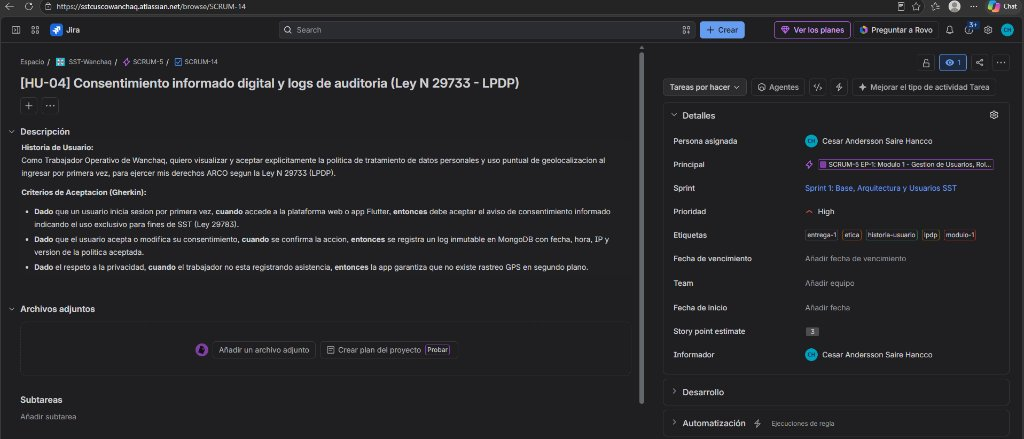
\includegraphics[width=\textwidth]{captura2_jira_hu_lpdp.jpg}
    \caption{Detalle de la Historia de Usuario \texttt{SCRUM-14} (\texttt{[HU-04]} --- Cumplimiento LPDP), evidenciando redacción ágil, criterios de aceptación Gherkin, Story Points, etiquetas y vinculación a \texttt{SCRUM-5}.}
    \label{fig:jira_hu}
\end{figure}

\subsubsection*{C. Requisitos No Funcionales (RNF)}

\begin{table}[H]
\centering
\caption{Requisitos No Funcionales (RNF) del sistema}
\label{tab:rnf}
\renewcommand{\arraystretch}{1.22}
\small
\begin{tabularx}{\textwidth}{C{1.5cm} L{3.3cm} Y}
\toprule
\rowcolor{PrimaryNavy}
\textcolor{white}{\textbf{Código}} & \textcolor{white}{\textbf{Categoría}} & \textcolor{white}{\textbf{Descripción del Requisito}} \\
\midrule
\textbf{RNF-01} & Seguridad y Cifrado & Comunicación cliente-servidor bajo HTTPS/TLS; contraseñas cifradas con \texttt{bcrypt}/\texttt{argon2} y sesiones JWT con expiración controlada. \\
\rowcolor{LightTint}
\textbf{RNF-02} & Privacidad y LPDP & Cumplimiento estricto de la Ley N.\textsuperscript{o} 29733 (LPDP): consentimiento expreso, derechos ARCO, minimización de datos y prohibición de rastreo GPS continuo en segundo plano. \\
\textbf{RNF-03} & Rendimiento & Tiempo de respuesta máximo de 2 segundos en endpoints críticos (validación QR y registro de asistencia) bajo concurrencia de una cuadrilla (50 usuarios simultáneos). \\
\rowcolor{LightTint}
\textbf{RNF-04} & Disponibilidad / Offline & La app móvil Flutter tolera cortes de conectividad en zonas de obra encolando registros cifrados localmente para sincronización automática al recuperar señal. \\
\textbf{RNF-05} & Usabilidad & Interfaz móvil de alto contraste y flujos de máximo 3 toques para facilitar su uso por personal operativo de campo con diversa alfabetización digital. \\
\rowcolor{LightTint}
\textbf{RNF-06} & Integridad Legal & Sellado temporal (\textit{timestamp}), código hash verificable y borrado lógico que garantiza la conservación auditable mínima de 5 años (D.S. N.\textsuperscript{o} 005-2012-TR). \\
\bottomrule
\end{tabularx}
\end{table}

\subsubsection*{D. Definition of Done (DoD) con Aspectos Éticos y Legales (LPDP)}

Una Historia de Usuario o tarea en Jira solo podrá transicionar al estado \textbf{``Done / Listo''} cuando cumpla simultáneamente con los siguientes criterios verificados por el Scrum Master y el Product Owner:

\begin{enumerate}[leftmargin=1.5em, itemsep=0.3em]
    \item \textbf{Criterios Técnicos y de Calidad de Código:}
    \begin{itemize}[leftmargin=1.2em]
        \item Código implementado bajo estándares de TypeScript (NestJS/React) y Dart (Flutter) sin errores de compilación ni advertencias críticas de linter.
        \item Commits enlazados explícitamente a la clave de Jira (ej. \texttt{SCRUM-11: Implementar guard JWT}) y Pull Request revisado y aprobado en GitHub.
        \item Pruebas unitarias y funcionales básicas ejecutadas exitosamente validando todos los Criterios de Aceptación (Gherkin).
    \end{itemize}
    \item \textbf{Criterios Éticos y Legales (Cumplimiento LPDP --- Ley N.\textsuperscript{o} 29733):}
    \begin{itemize}[leftmargin=1.2em]
        \item \textit{Consentimiento y Finalidad:} Ningún formulario recopila datos personales innecesarios; los datos del trabajador (DNI, nombre, área) se utilizan únicamente para acreditación de SST bajo consentimiento informado registrado.
        \item \textit{Privacidad de Geolocalización:} Se verifica en pruebas móviles que el permiso GPS se invoca únicamente durante el marcado puntual de asistencia y se libera de inmediato (cero vigilancia encubierta).
        \item \textit{Seguridad y Confidencialidad:} No existen credenciales, claves API ni datos personales reales expuestos en el repositorio público de GitHub (uso de \texttt{.env} y datos sintéticos/anonimizados para pruebas).
        \item \textit{Equidad e Inclusión:} Interfaz accesible y liviana compatible con dispositivos Android de gama baja/media utilizados por personal operativo.
    \end{itemize}
    \item \textbf{Criterios de Gestión y Documentación:}
    \begin{itemize}[leftmargin=1.2em]
        \item Documentación técnica y diagramas UML impactados actualizados.
        \item Historia validada y aprobada por el Product Owner en Jira con evidencia adjunta.
    \end{itemize}
\end{enumerate}

\subsection*{2.2. Planificación de Sprints}
\addcontentsline{toc}{subsection}{2.2. Planificación de Sprints}

El proyecto se organiza en \textbf{4 Sprints} que cubren las 16 semanas del semestre académico, alineados a los tres entregables establecidos en el sílabo (Tabla~\ref{tab:sprints}).

\begin{table}[H]
\centering
\caption{Planificación preliminar de Sprints y entregables del proyecto}
\label{tab:sprints}
\renewcommand{\arraystretch}{1.22}
\footnotesize
\begin{tabularx}{\textwidth}{L{1.8cm} C{1.7cm} Y C{2.1cm} C{1.0cm} L{3.2cm}}
\toprule
\rowcolor{PrimaryNavy}
\textcolor{white}{\textbf{Sprint}} & \textcolor{white}{\textbf{Periodo}} & \textcolor{white}{\textbf{Objetivo del Sprint}} & \textcolor{white}{\textbf{Historias}} & \textcolor{white}{\textbf{SP}} & \textcolor{white}{\textbf{Entregable Asociado}} \\
\midrule
\textbf{Sprint 1} \textit{(Activo)} & Sem. 1--2 & Planificación Scrum, arquitectura base, DoD (LPDP), autenticación JWT y gestión inicial de personal y sedes de Wanchaq. & HU-01 a HU-04 & 16 & \textbf{Entrega N.\textsuperscript{o} 1 (Sem. 2):} Cap. I, Bosquejo Cap. II y Backlog en Jira. \\
\rowcolor{LightTint}
\textbf{Sprint 2} \textit{(Planif.)} & Sem. 3--6 & Núcleo web y móvil: catálogo SST (Ley 29783), programación de sesiones y asistencia en campo con QR dinámico y geocerca GPS. & HU-05 a HU-10 & 34 & \textbf{Entrega N.\textsuperscript{o} 2 (Sem. 6):} Cap. I--III parcial + \textbf{Sistema al 50\%}. \\
\textbf{Sprint 3} \textit{(Backlog)} & Sem. 7--11 & Portal móvil del trabajador, notificaciones push, evaluaciones automatizadas y generación de certificados PDF verificables con QR. & HU-11 a HU-14 & 21 & Incremento funcional (80\%): App Capacitando y Certificados QR. \\
\rowcolor{LightTint}
\textbf{Sprint 4} \textit{(Backlog)} & Sem. 12--16 & Dashboard gerencial SST, alertas Ley 29783, exportación R.M. 050-2013-TR, impacto sostenible, pruebas finales y despliegue Cloud. & HU-15 a HU-18 & 21 & \textbf{Entrega N.\textsuperscript{o} 3 (Sem. 16):} Informe Final (Cap. I--VII) + \textbf{Sistema 100\% Cloud}. \\
\bottomrule
\end{tabularx}
\end{table}

\begin{figure}[H]
    \centering
    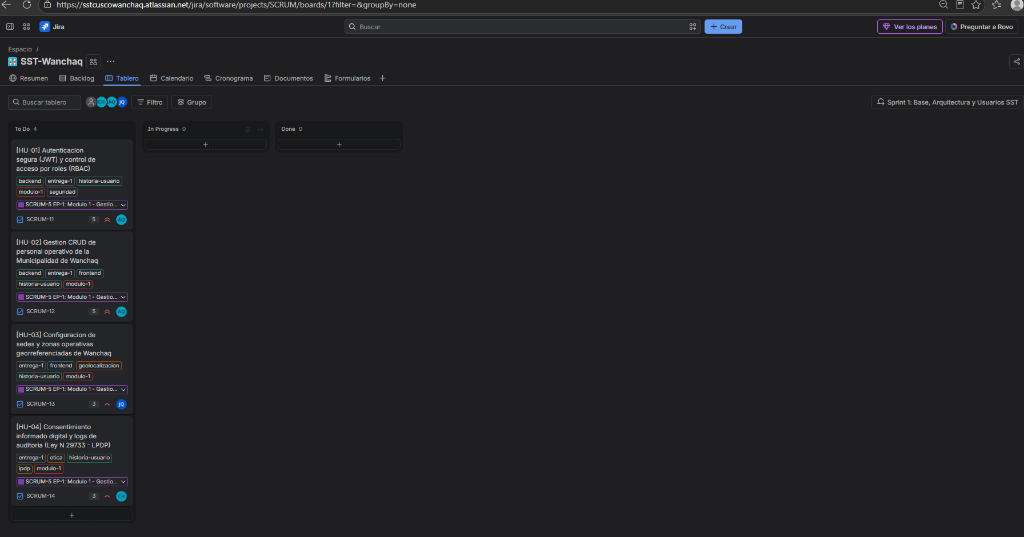
\includegraphics[width=\textwidth]{captura3_jira_tablero_sprint1.png}
    \caption{Tablero Scrum activo del Sprint 1 (\textit{Base, Arquitectura y Usuarios SST}) en Jira Software con las historias \texttt{SCRUM-11} a \texttt{SCRUM-14}.}
    \label{fig:jira_board}
\end{figure}

\subsection*{2.3. Herramientas de Colaboración Utilizadas}
\addcontentsline{toc}{subsection}{2.3. Herramientas de Colaboración Utilizadas}

Para garantizar trazabilidad, transparencia y trabajo colaborativo entre los 4 integrantes se emplean las siguientes herramientas integradas:

\begin{enumerate}[leftmargin=1.5em, itemsep=0.25em]
    \item \textbf{Jira Software Cloud (\url{https://sstcuscowanchaq.atlassian.net}):} Gestión centralizada del Product Backlog, Épicas, Historias de Usuario, Story Points, asignación de responsables y monitoreo de Sprints.
    \item \textbf{GitHub (\url{https://github.com/141158/sst-wanchaq-platform}):} Control de versiones distribuido mediante ramas por historia (\texttt{feature/SCRUM-XX-descripcion}) y revisión de código por Pull Requests.
    \item \textbf{Integración Jira + GitHub (\textit{GitHub for Jira}):} Vinculación bidireccional activa que enlaza automáticamente los commits y Pull Requests de GitHub dentro de cada tarjeta de Jira, como se evidencia en las Figuras~\ref{fig:github_repo} y~\ref{fig:jira_github}.
    \item \textbf{Figma:} Diseño colaborativo de prototipos UI/UX de la plataforma web y la aplicación móvil Flutter.
    \item \textbf{Discord / WhatsApp:} Coordinación ágil de los \textit{Daily Scrums} (15 minutos), resolución de impedimentos y preparación de \textit{Sprint Reviews}.
\end{enumerate}

\begin{figure}[H]
    \centering
    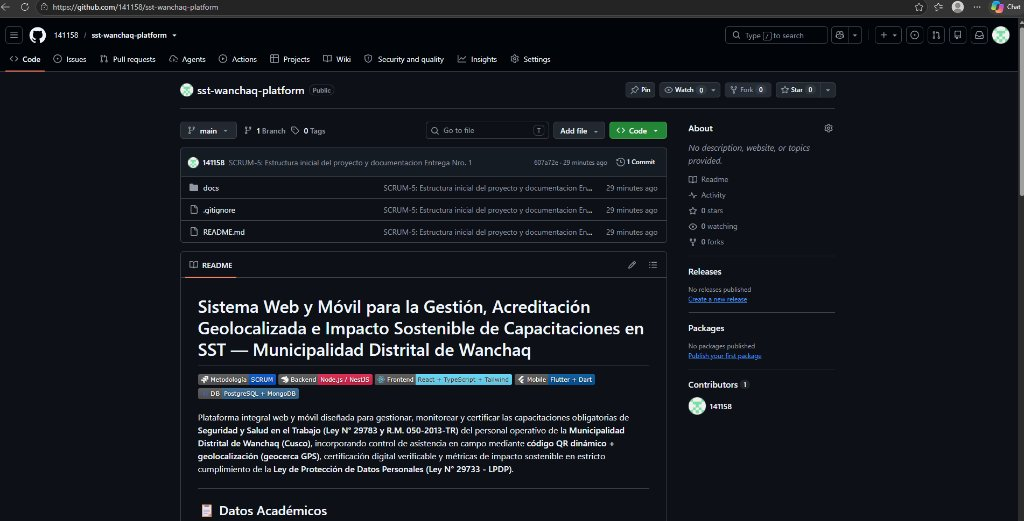
\includegraphics[width=\textwidth]{captura4_github_repositorio.jpg}
    \caption{Repositorio oficial del proyecto en GitHub (\texttt{141158/sst-wanchaq-platform}) con la documentación inicial y el primer commit enlazado a \texttt{SCRUM-5}.}
    \label{fig:github_repo}
\end{figure}

\begin{figure}[H]
    \centering
    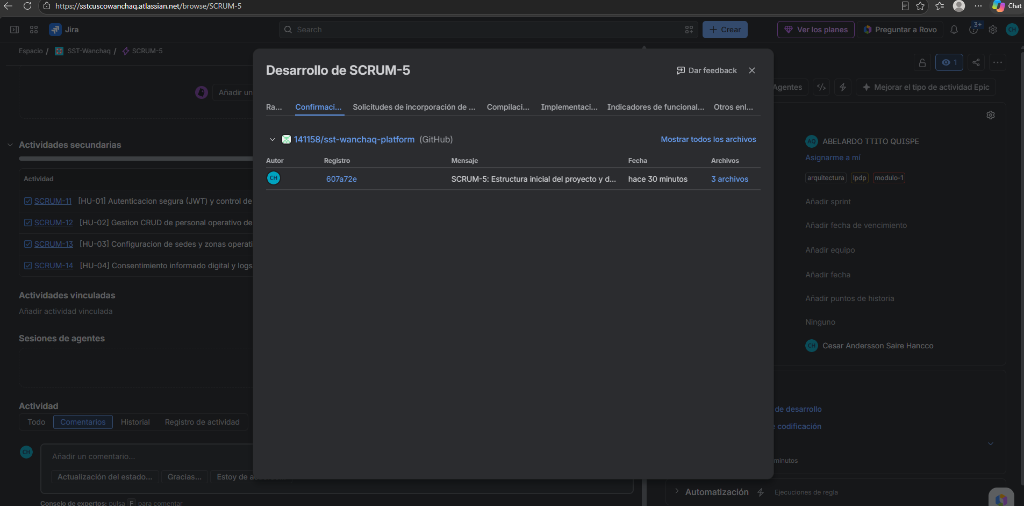
\includegraphics[width=\textwidth]{captura5_jira_github_integracion.png}
    \caption{Panel de Desarrollo en Jira (\texttt{SCRUM-5}) evidenciando la sincronización automática del commit \texttt{607a72e} proveniente del repositorio GitHub.}
    \label{fig:jira_github}
\end{figure}

\end{document}
